\documentclass[12pt,a4paper]{article}
% Packages nécessaires
\usepackage[utf8]{inputenc}
\usepackage[T1]{fontenc}
\usepackage[french]{babel}
\usepackage{graphicx}
\usepackage{amsmath}
\usepackage{geometry}
\usepackage{float}
\usepackage{enumitem}
\usepackage{setspace}
\usepackage{titlesec}
\usepackage{url}
\usepackage{natbib}
\usepackage{hyperref}
\usepackage{tocloft}
\usepackage{bookmark}

% Configuration des marges et de l'espacement
\geometry{margin=2.5cm}
\onehalfspacing

% Supprimer le retrait automatique des paragraphes
\setlength{\parindent}{0pt}

% Si vous souhaitez ajouter un espace entre les paragraphes (optionnel)
\setlength{\parskip}{6pt}

% Personnalisation des titres
\titleformat{\section}{\normalfont\large\bfseries}{\thesection}{1em}{}
\titleformat{\subsection}{\normalfont\normalsize\bfseries}{\thesubsection}{1em}{}

% Configuration du titre principal (centré comme dans le document original)
\title{
\vspace{2cm}
\Large\textbf{GLACIES - Global Low-orbit Arctic Cryosphere Imaging and Environmental Surveillance\\
Exercice Pratique 4 --- GEO1117 \\
Capteurs et sources de données}
\vspace{1cm}
}

\author{Thierry Laurent St-Pierre}
\date{
20 mars 2025\\
\vspace{1cm}
À remettre le 4 avril 2025
}

% Configuration des liens hypertextes
\hypersetup{
    colorlinks=true,
    linkcolor=blue,
    filecolor=magenta,
    urlcolor=cyan,
    breaklinks=true  % Permet aux liens de se couper sur plusieurs lignes
}

% Améliore la gestion des URLs
\urlstyle{same}
\Urlmuskip=0mu plus 1mu

\begin{document}

\maketitle

\tableofcontents
\thispagestyle{empty}
\newpage

\subsection{Images satellitaires 1}

\begin{figure}[H]
    \centering
    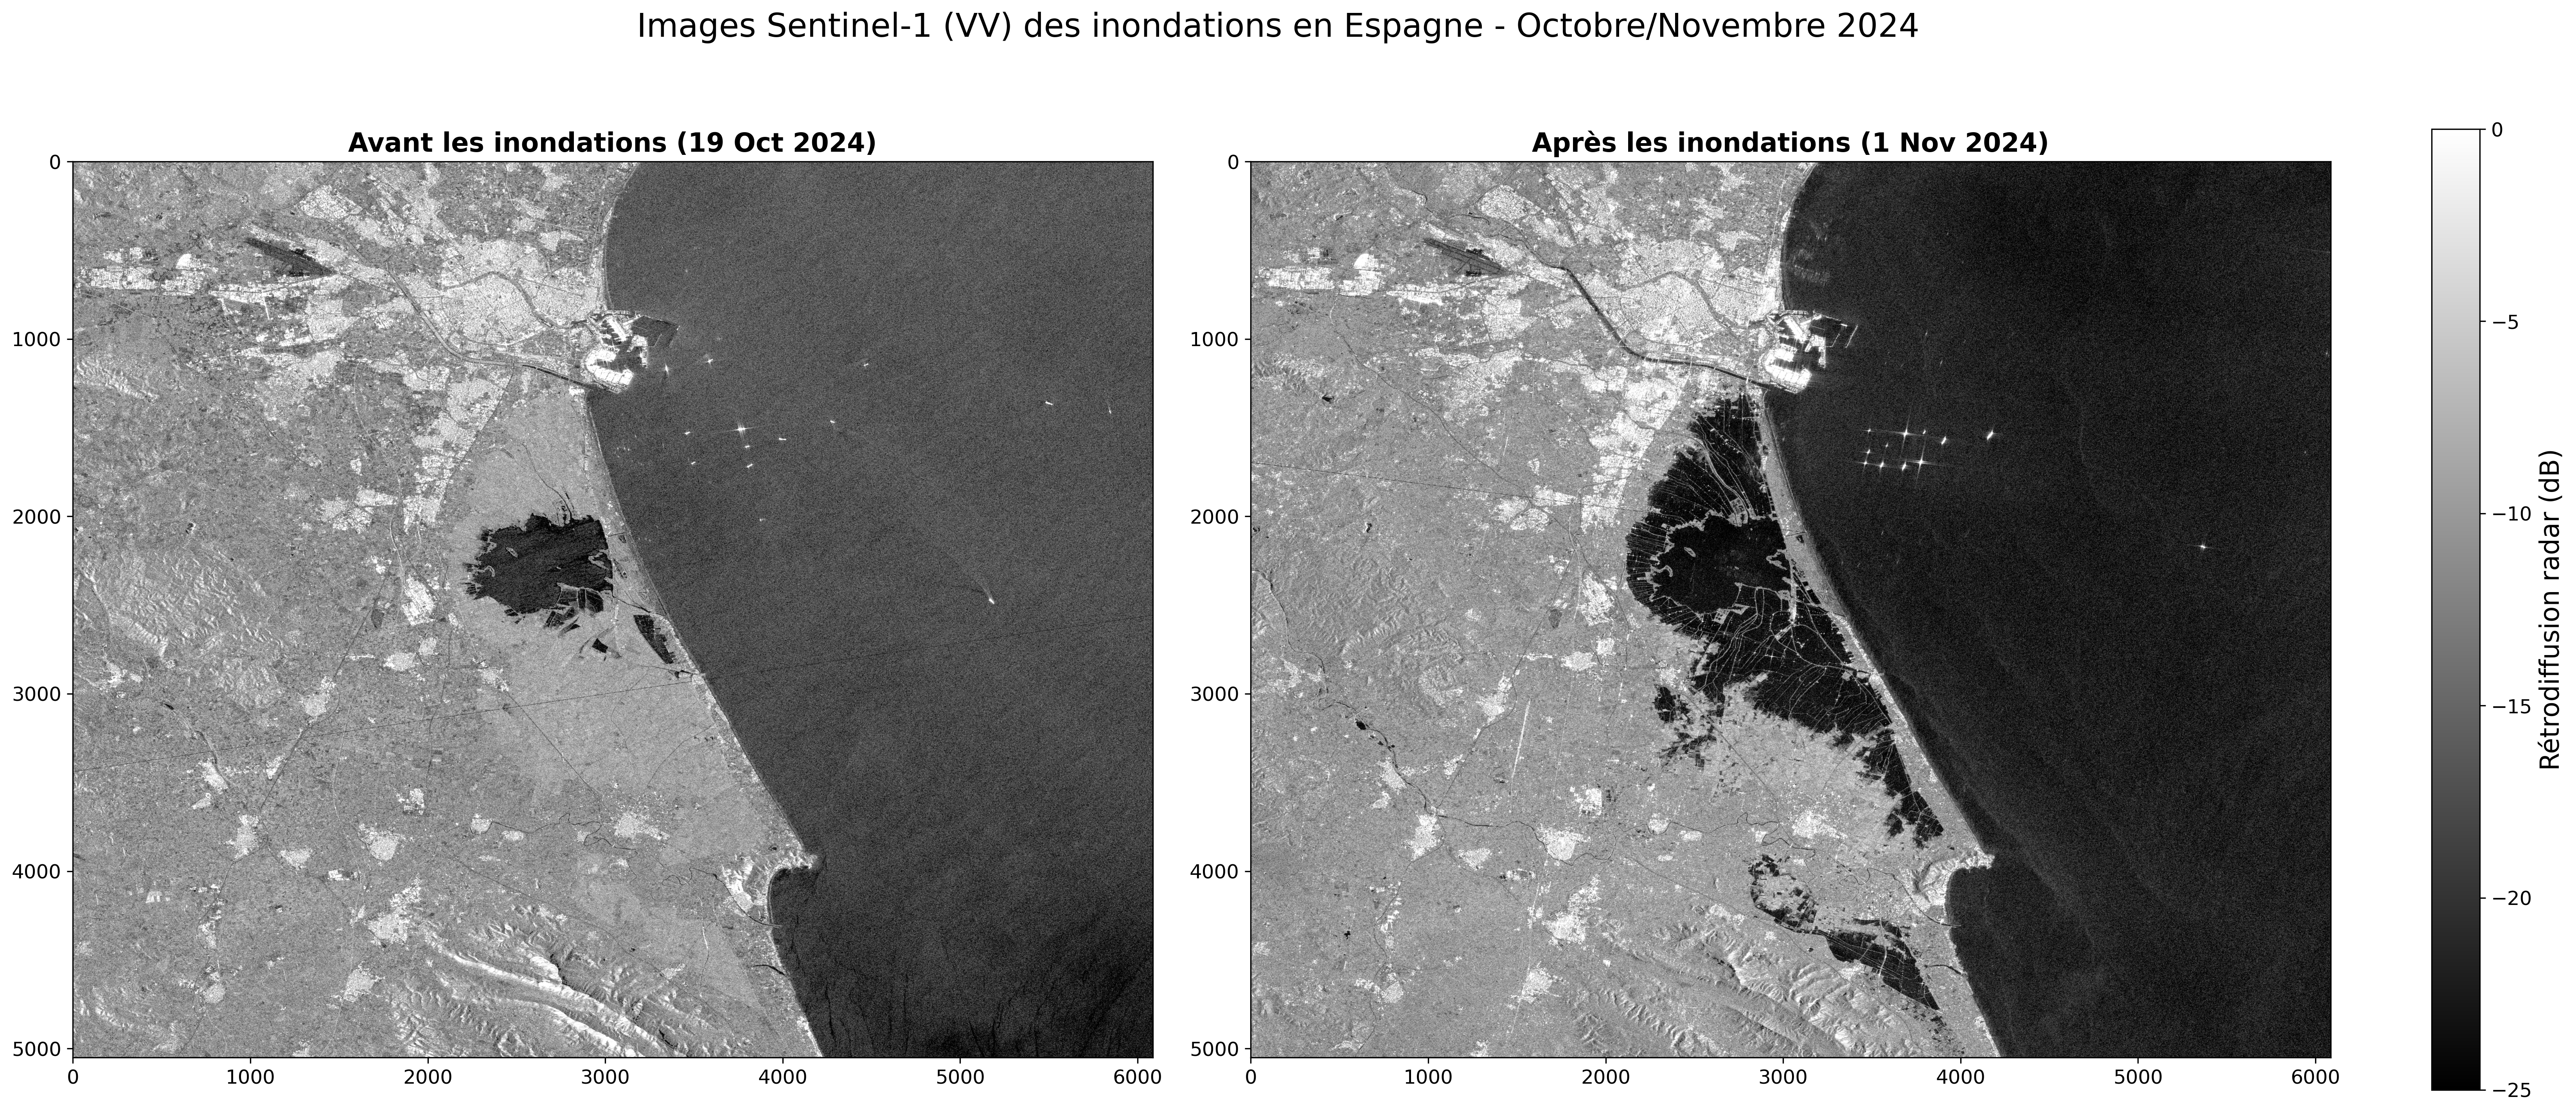
\includegraphics[width=1\textwidth]{Comparaison_Inondations_Espagne.png}
    \caption{Inondations dans la région de Valence, Espagne, comparaison entre le 19 octobre et le 1er novembre 2024, captée par Sentinel-1}
    \label{fig:image1}
\end{figure}

\textbf{Analyse d'inondations par imagerie radar Sentinel-1}

L'image 1 montre les inondations catastrophiques survenues fin octobre 2024 dans la région de Valence en Espagne \citep{ESA2024}, capturées grâce au satellite Sentinel-1 de l'Agence Spatiale Européenne (ESA). 

Ce satellite embarque un Radar à Synthèse d'ouverture (SAR) en bande C qui opère à une longueur d'onde d'environ 5,6 cm \citep{ESA2023}. Les images présentées ont été acquises à deux dates distinctes : le 19 octobre 2024 (avant inondation) et le 1er novembre 2024 (après inondation), avec une polarisation VV et une résolution spatiale de 10 mètres. Sentinel-1A suit une orbite héliosynchrone quasi-polaire à 693 km d'altitude, effectuant 175 orbites par cycle de répétition de 12 jours. La constellation complète, composée des satellites Sentinel-1A et Sentinel-1B partageant le même plan orbital, offre une résolution temporelle améliorée de 6 jours.

La technologie radar utilisée repose sur le principe de rétrodiffusion des micro-ondes. Le capteur émet des ondes polarisées qui interagissent avec la surface terrestre selon leurs propriétés diélectriques et leur rugosité. Les surfaces d'eau calme agissent comme des miroirs, réfléchissant l'onde radar loin du capteur, ce qui crée des zones très sombres (faible rétrodiffusion) sur l'image 1. À l'inverse, les zones urbaines, les structures et les embarcations produisent de multiples réflexions en coin qui renvoient fortement le signal vers le capteur, apparaissant en blanc. Les zones en gris correspondent à des terres agricoles, de la végétation ou des sols nus dont la rugosité génère une rétrodiffusion de surface modérée.

Le capteur utilise la méthode d'acquisition TOPSAR (Terrain Observation with Progressive Scans SAR), une technique d'imagerie ScanSAR où les données sont acquises par rafales en commutant cycliquement le faisceau d'antenne entre plusieurs sous-fauchées adjacentes. Cette approche permet de couvrir une large fauchée atteignant 250 km en mode Interferometric Wide Swath (IW).

La comparaison des deux images montre une nette expansion des zones noires sur l'image du 1er novembre, correspondant aux terres tout récemment submergées et absentes de l'image du 19 octobre. Cette différence de signature de rétrodiffusion entre les deux dates a permis de cartographier avec précision l'étendue des inondations. Selon l'analyse des images Sentinel-1 et Sentinel-2 réalisée par l'ESA, environ 15 633 hectares de terres ont été inondés dans la province de Valence \citep{ESA2024}.

Un avantage majeur de la télédétection radar pour le suivi des inondations est dans sa capacité à acquérir des images indépendamment des conditions d'illumination (jour/nuit) et météorologiques. Contrairement aux capteurs optiques passifs, le radar peut pénétrer les nuages, ce qui permet ainsi une surveillance continue même dans des conditions non optimales.

\subsection{Images satellitaires 2}

\begin{figure}[H]
    \centering
    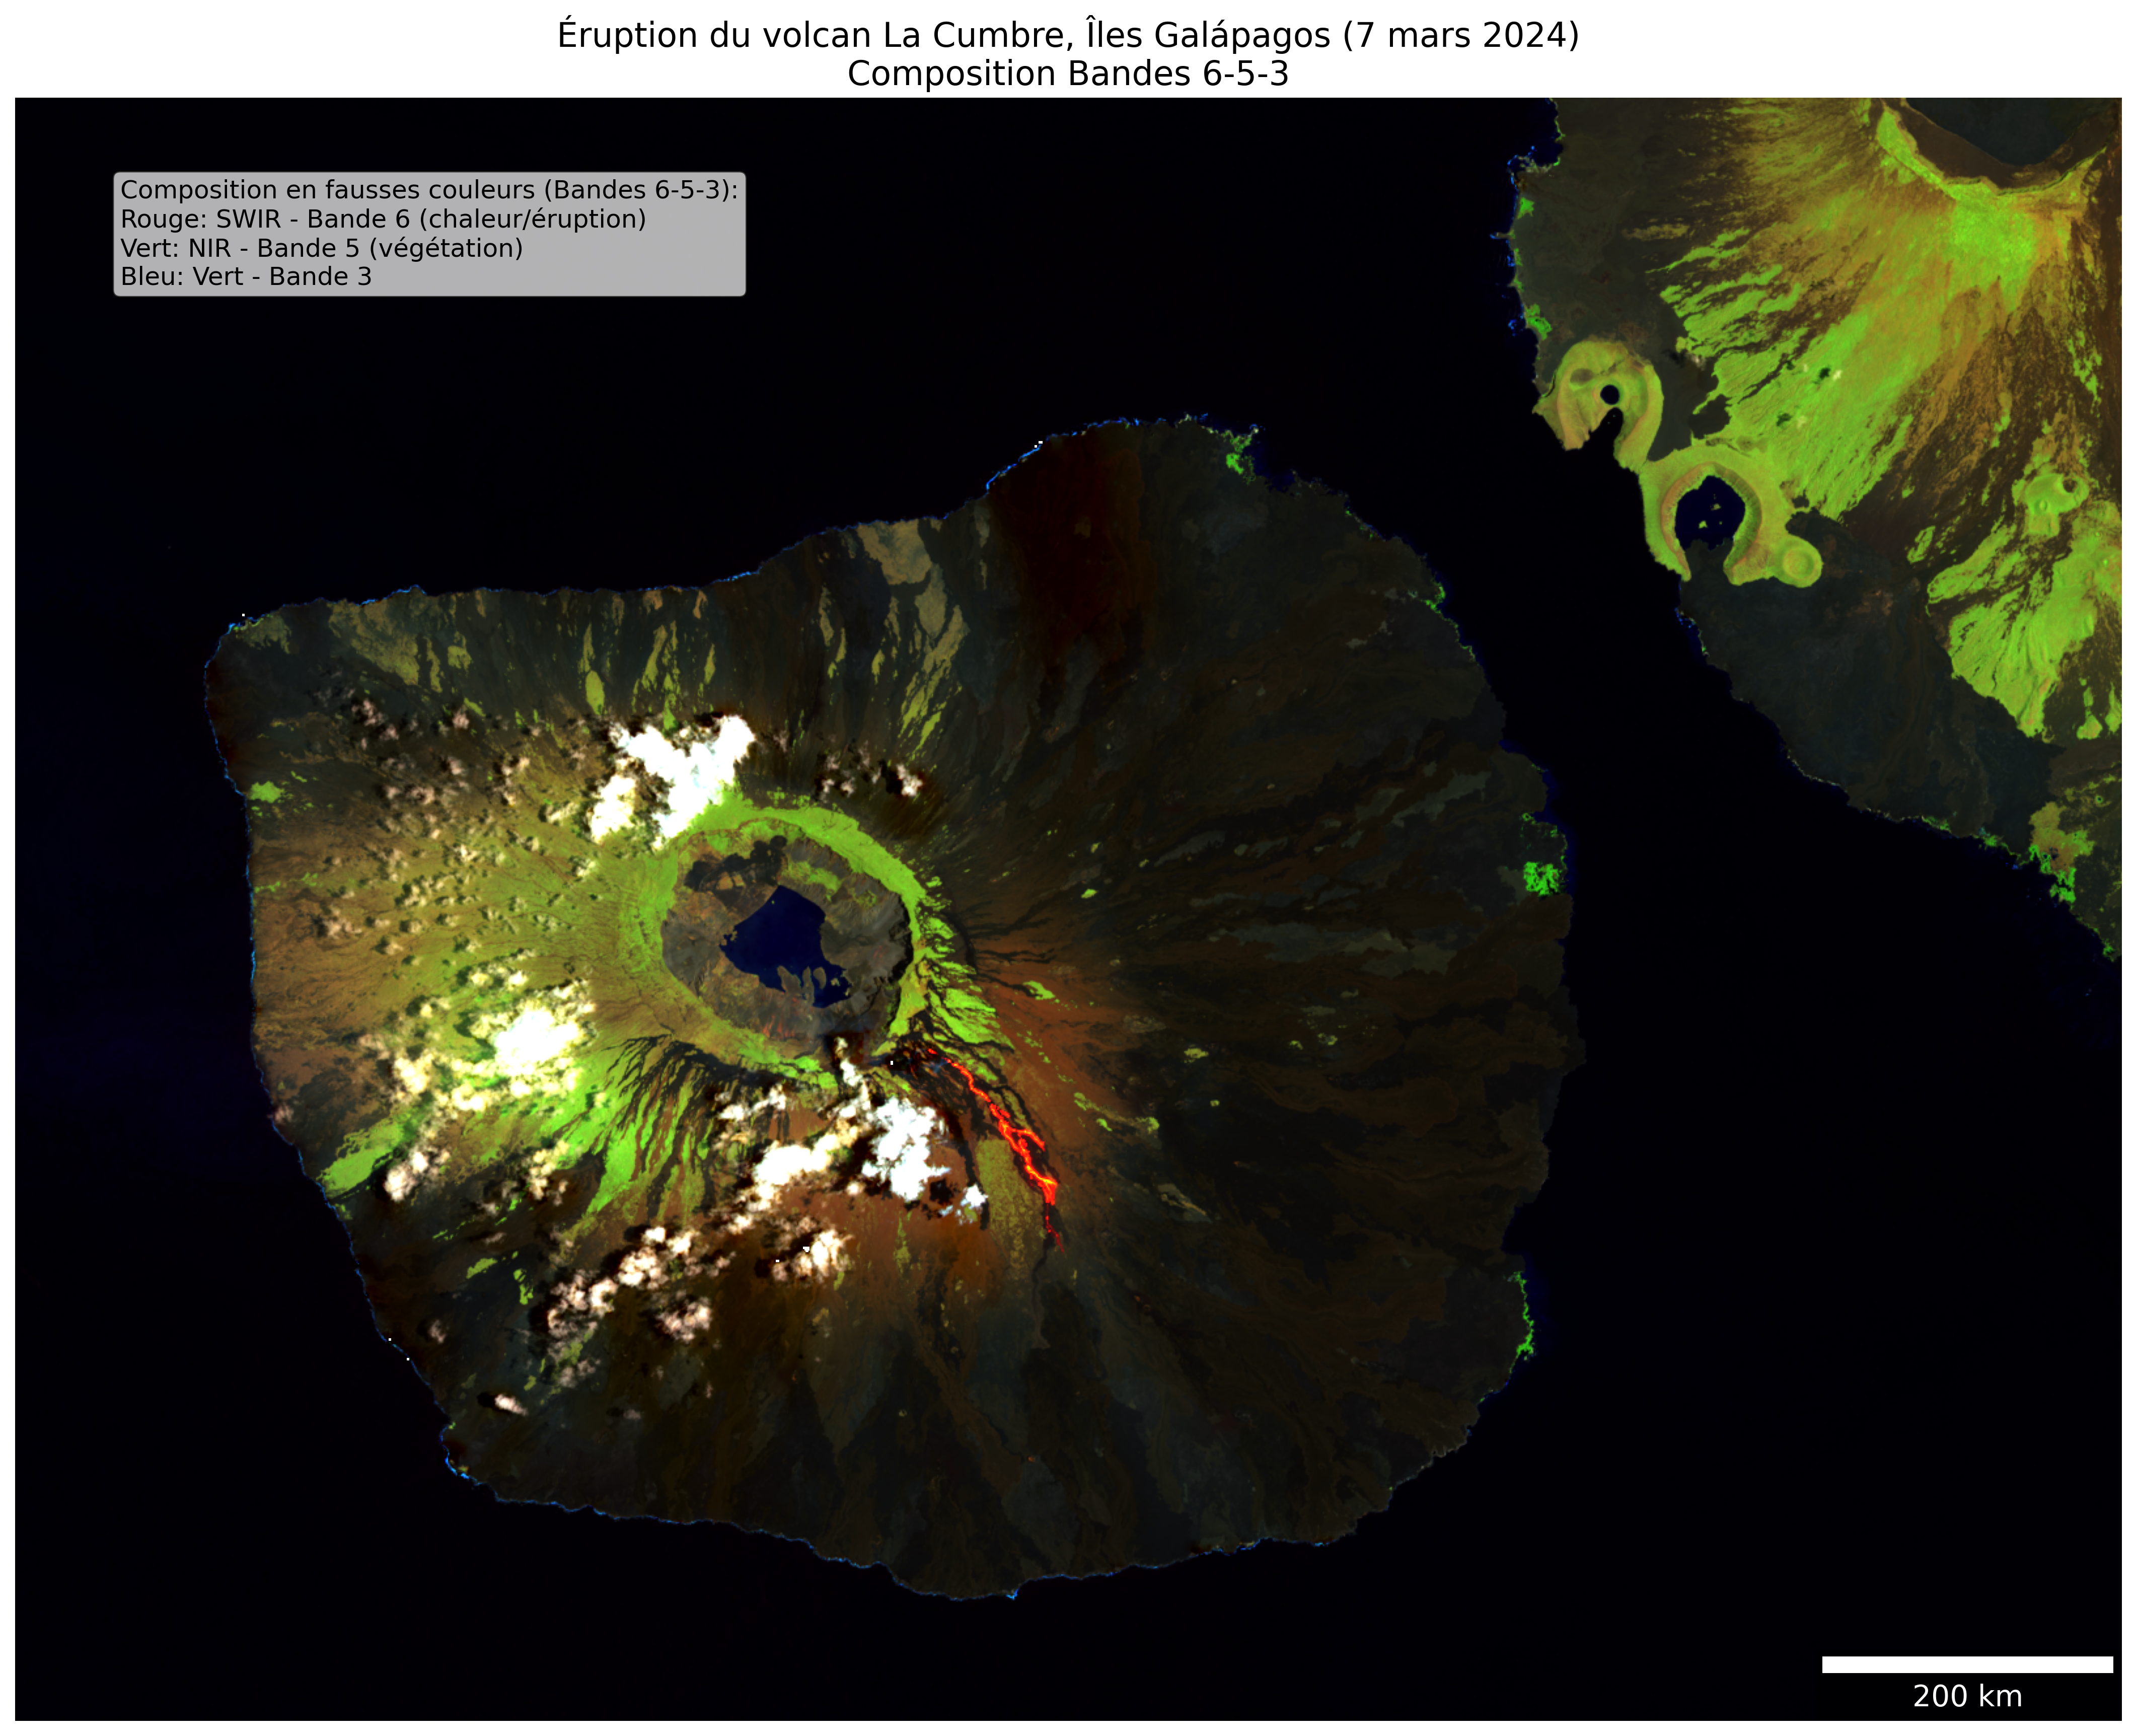
\includegraphics[width=1\textwidth]{Volcan_LaCumbre_Rasterio_Show.png}
    \caption{Éruption du volcan La Cumbre sur l'île Fernandina, archipel des Galápagos, 7 mars 2024, captée par Landsat 8 en composition colorée 6-5-3}
    \label{fig:image2}
\end{figure}

\textbf{Analyse d'une éruption volcanique par imagerie multispectrale Landsat 8}

L'image 2 montre l'éruption du volcan La Cumbre sur l'île Fernandina dans l'archipel des Galápagos \citep{NASA2024}. L'activité volcanique, débutée le 2 mars 2024, a été observée le 7 mars 2024 grâce au satellite Landsat 8 et son capteur optique multispectral OLI/TIRS (Operational Land Imager/Thermal Infrared Sensor).

Ce système de télédétection, opéré conjointement par la NASA et l'USGS \citep{USGS2022}, embarque un capteur multispectral qui offre une résolution spatiale de 30 mètres pour les bandes visibles et proche infrarouge (NIR), 15 mètres pour la bande panchromatique, et 100 mètres pour les bandes thermiques (TIRS). Sa résolution spectrale est remarquable avec 11 bandes couvrant un spectre électromagnétique allant du visible à l'infrarouge thermique. Le satellite Landsat 8 suit une orbite héliosynchrone à 705 km d'altitude avec une inclinaison de 98,2 degrés, ce qui permet une couverture complète de la Terre tous les 16 jours (résolution temporelle).

L'image est présentée en composition colorée 6-5-3 (SWIR-NIR-Vert), spécialement choisie pour mettre en évidence l'activité volcanique. Les coulées de lave récentes apparaissent en rouge/orange vif, conséquence directe de leur forte émission thermique captée dans la bande 6 (SWIR, 1.57-1.65 \textmu m). Cette détection s'appuie sur la loi de Planck qui régit l'émission électromagnétique des corps chauds, dont le pic d'émission se déplace vers les longueurs d'onde plus courtes à mesure que la température augmente. La technologie d'acquisition "pushbroom" employée par Landsat 8, qui représente une évolution par rapport aux scanners à miroir tournant des générations précédentes, permet de capturer des images sur une fauchée de 185 km de large en un seul passage, offrant ainsi une vue complète du phénomène volcanique.

Dans cette composition colorée, la végétation de l'île se distingue par sa teinte vert vif, résultat de sa haute réflectance dans la bande 5 (NIR, 0.85-0.88 \textmu m). Cette forte réflexion dans le proche infrarouge est due à la structure cellulaire des feuilles et à la diffusion interne du rayonnement au sein des tissus végétaux. Le cratère central du volcan apparaît en bleu foncé/noir, traduisant l'absence de végétation et une faible réflectance dans les trois bandes utilisées. Les zones blanches visibles correspondent à des nuages ou à des émissions de vapeur et de cendres volcaniques qui réfléchissent fortement le rayonnement dans l'ensemble des bandes spectrales utilisées.

Cette application de la télédétection exploite les principes fondamentaux des capteurs passifs qui mesurent à la fois le rayonnement solaire réfléchi (dans les domaines du visible et du proche infrarouge) et le rayonnement émis par les surfaces terrestres (particulièrement dans l'infrarouge à ondes courtes). Cette capacité d'observation à distance permet de surveiller en toute sécurité des phénomènes naturels potentiellement dangereux comme les éruptions volcaniques, illustrant parfaitement l'intérêt stratégique de la télédétection pour la gestion des risques naturels et l'étude des processus géophysiques actifs.

\subsection{Proposition de mission satellitaire}
\begin{itemize}[label=---]
    \item \textbf{Phénomène à observer :}
    
    La surveillance des changements de la banquise arctique. C'est un phénomène important pour le suivi du changement climatique et particulièrement pertinent pour le Canada qui possède une grande partie du territoire arctique \citep{Derksen2019}.
    
    \item \textbf{Longueur(s) d'onde proposée(s) :}
        
    Pour observer efficacement la banquise, les micro-ondes actives (radar à synthèse d'ouverture ou SAR) dans les bandes C (5,3 GHz) et X (9,6 GHz) \citep{Liu2023}, les micro-ondes passives dans la gamme 6-37 GHz \citep{Webster2023}, et l'infrarouge thermique (10-12 $\mu$m) pour mesurer la température de surface. Les micro-ondes sont particulièrement adaptées car elles peuvent pénétrer les nuages et fonctionner indépendamment des conditions d'illumination, ce qui est crucial dans les régions polaires où l'obscurité hivernale est prolongée.
    
    \item \textbf{Résolutions requises :}
    
    La résolution spatiale idéale serait de 10-30 m pour le SAR afin d'obtenir des détails fins de la glace, et de 1-5 km pour les micro-ondes passives permettant une couverture plus large. Pour la résolution temporelle, un intervalle de 1-3 jours serait optimal pour suivre la dynamique rapide de la banquise, particulièrement pendant les périodes de fonte ou de formation de glace.
\end{itemize}

\subsection{Types d'orbites}
\begin{itemize}[label=---]
    \item \textbf{Explication des deux types d'orbite principaux :}
    
    \item \textbf{Orbite géostationnaire (GEO):} Située à environ 36 000 km d'altitude au-dessus de l'équateur, avec une période orbitale de 24 heures synchronisée avec la rotation terrestre \citep{Weather2023, Capderou2014}. Le satellite reste fixe par rapport à un point sur Terre, permettant une observation continue d'une même région. Avantages: couverture constante d'une large zone, acquisition en temps réel. Limitations: résolution spatiale réduite due à la grande altitude, couverture inefficace des régions polaires, coût de lancement élevé. Applications: météorologie opérationnelle, télécommunications, surveillance à grande échelle.
    
    \item \textbf{Orbite héliosynchrone (Sun-synchronous orbit ou SSO):} Type spécial d'orbite polaire ou quasi-polaire où le satellite passe au-dessus de chaque point de la Terre à la même heure locale à chaque passage. Typiquement à une altitude de 600-800 km. Avantages: conditions d'éclairement constantes facilitant la comparaison d'images dans le temps, bonne résolution spatiale, couverture globale incluant les pôles. Limitations: revisite moins fréquente pour un point donné (généralement quelques jours), acquisition non continue. Applications: cartographie, suivi environnemental, agriculture, foresterie, et la plupart des missions d'observation terrestre.
    
    \item \textbf{Type d'orbite le mieux adapté à ma mission GLACIES :}
    
    Pour la mission GLACIES de surveillance de la banquise arctique, l'orbite héliosynchrone est clairement la plus adaptée. Elle permet une couverture efficace des régions polaires, offre une résolution spatiale suffisante pour détecter les détails de la glace de mer, et fournit des conditions d'illumination constantes qui facilitent l'analyse comparative des données dans le temps. De plus, en utilisant plusieurs satellites sur la même orbite mais avec des plans orbitaux décalés (constellation), nous pouvons atteindre une revisite fréquente (1-3 jours) nécessaire pour suivre la dynamique rapide de la banquise, tout en conservant les avantages de l'orbite héliosynchrone.
\end{itemize}

\subsection{Questions des médias}
\begin{itemize}[label=---]
    \item \textbf{Satellite présentement en orbite pour le suivi de la banquise :}
    
    Le satellite RADARSAT Constellation Mission (RCM) du Canada est mon choix principal pour le suivi de la banquise arctique \citep{CSA2019, Zakhvatkina2022}. Cette mission, lancée en 2019, comprend trois satellites SAR en orbite quasi-polaire avec un déphasage de 120° entre eux. RCM est spécifiquement conçue pour la surveillance des régions arctiques canadiennes avec une résolution spatiale de 5 à 100 mètres selon les modes d'acquisition. La constellation permet une revisite quotidienne de l'Arctique et dispose de modes d'acquisition adaptés à la détection des types de glace et au suivi des déplacements de la banquise. Ses capacités SAR en bande C sont idéales pour observer la glace indépendamment des conditions météorologiques et d'illumination.
    
    \item \textbf{Options de décommission du satellite :}
    
    Deux options vraisemblables pour limiter les débris spatiaux produits par la mission GLACIES seraient :
    
    1) La rentrée atmosphérique contrôlée, en programmant le satellite pour qu'il descende dans l'atmosphère terrestre selon une trajectoire précise. Il se désintégrerait majoritairement lors de la rentrée avec les éventuels débris tombant dans des zones océaniques inhabitées. Cette méthode est particulièrement adaptée pour les satellites en orbite basse comme ceux de la mission GLACIES.
    
    2) Pour les composants qui ne se désintégreraient pas complètement, l'autre option serait de concevoir le satellite selon les principes de "Design for Demise", en utilisant des matériaux qui se consumeraient entièrement lors de la rentrée atmosphérique \citep{NASA2023, IADC2020} et en intégrant des mécanismes de passivation (vidange des réservoirs, décharge des batteries) conformément aux directives internationales de mitigation des débris spatiaux \citep{Dutta2022}.
\end{itemize}

\subsection{Bonus - Nom de la mission}
\textbf{Acronyme et nom de la mission :}
GLACIES - Global Low-orbit Arctic Cryosphere Imaging and Environmental Surveillance. Ce nom fait référence à la surveillance de la cryosphère (la glace terrestre) en mettant l'accent sur l'Arctique, tout en suggérant une portée globale pour les implications environnementales des données recueillies. De plus, "glacies" signifie "glace" en latin, ce qui renforce la thématique de la mission.

\newpage
\bibliographystyle{plainnat}
\bibliography{references_corrected_updated}

\newpage
\subsection*{Codes source et ressources supplémentaires}

Les images et analyses présentées dans ce rapport ont été réalisées à l'aide de la plateforme Google Earth Engine. Les codes sources utilisés pour le traitement des images sont disponibles aux liens suivants :

\begin{itemize}
    \item Code pour l'analyse des inondations en Espagne (Sentinel-1): 
    \url{https://code.earthengine.google.com/?scriptPath=users/thierry-laurent/teledetection:inondations_valence_espagne}
    
    \item Code pour l'analyse de l'éruption volcanique La Cumbre (Landsat 8): 
    \url{https://code.earthengine.google.com/?scriptPath=users/thierry-laurent/teledetection:volcan_lacumbre_galapagos}
\end{itemize}

Notes : Les URL ci-dessus sont des exemples. Vous pouvez les remplacer par les liens réels vers vos scripts Google Earth Engine.

\end{document}